
\section{Implementation}
\label{sec:impl}

We now describe the implementation of the \ix prototype. We start with
an overview of the system itself, including the separation of control
plane and dataplane, the use of virtualization hardware for
protection, and resource allocation (\S\ref{sec:impl:overview}). We
then describe salient aspects of our system, including the internals
of the \ix kernel and in particular its pipeline
(\S\ref{sec:impl:kernel}), the native API at the kernel/user boundary
(\S\ref{sec:impl:api}), our approach to compatibility
(\S\ref{sec:impl:libix}), and finally our approach to flow control and
congestion management (\S\ref{sec:impl:net}).  We close with a
discussion of our approach, its current implementation restrictions,
and directions for future work (\S\ref{sec:impl:discussion}).


\subsection{Overview}
\label{sec:impl:overview}

\paragraph{System Architecture}

\begin{figure}
\begin{centering}
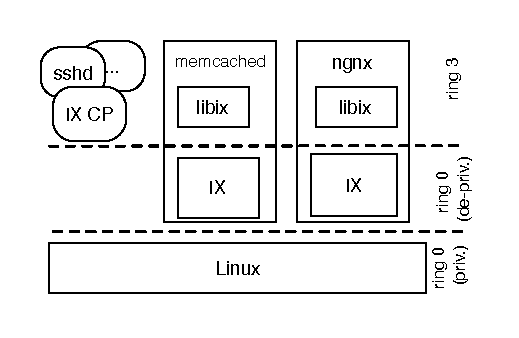
\includegraphics{figs/cp-dp.eps}
\centering\caption{Protection and separation in \ix.}
\label{fig:cp-dp}
\end{centering}
\end{figure}



\paragraph{Protection using hardware virtualization}


\paragraph{Multi-Queue and Bonding}

\begin{figure}
\hspace*{-0.25in}\centering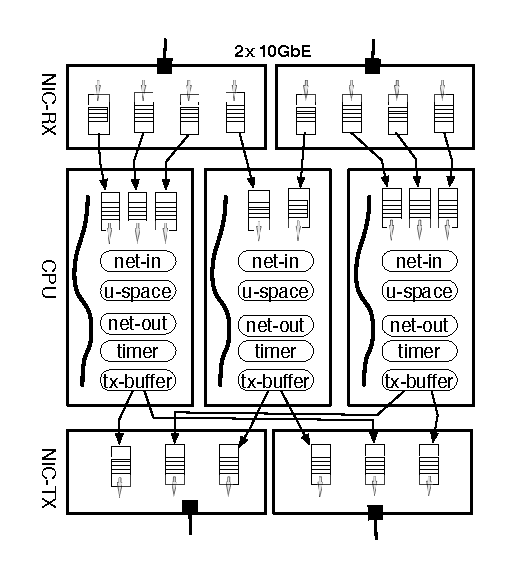
\includegraphics{figs/queues-cores.eps}
\caption{Example of IX scaling across two NICs interfaces, 8 NIC RX queues, and 3 CPU hardware threads.} 
\label{fig:queues-cores}
\end{figure}


%\begin{figure}
\begin{centering}
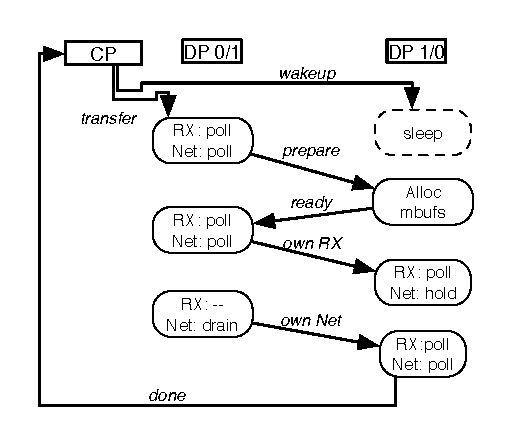
\includegraphics{figs/queue-takeover.eps}
\caption{Queue takeover algorithm.}
\label{fig:queue-takeover}
\end{centering}
\end{figure}




\paragraph{Resource allocation}


\subsection{The \ix Pipeline}
\label{sec:impl:kernel}

%\begin{figure}
\begin{centering}
% FIXME
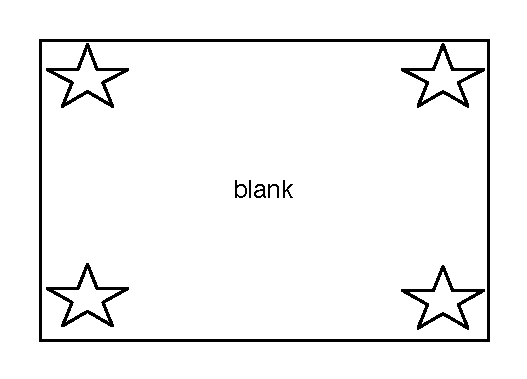
\includegraphics{figs/blank.eps}
\caption{Main stages of the \ix pipeline.}
\label{fig:pipeline}
\end{centering}
\end{figure}



\todo   Describe the pipeline stages from Fig~\ref{fig:queues-cores}
\todo   batching, stage, main loop, ...
\todo   hardware optimization
\todo   the driver layer
\todo   TCP processing
     
\subsection{The \ix native API}
\label{sec:impl:api}

\begin{figure}
\begin{centering}
% FIXME
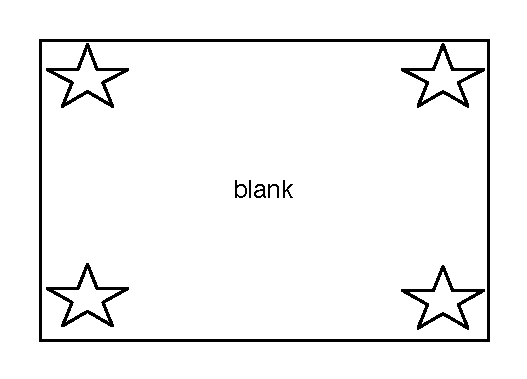
\includegraphics{figs/blank.eps}
\caption{Zero-copy, event-driven ping-pong server using the native \ix API.}
\label{fig:listing}
\end{centering}
\end{figure}


\todo Fig.~\ref{fig:listing} Listing .. (echo server)
\todo list of events (is it like Megapipe and/or mTCP)
\todo  true zero-copy

\subsection{LibEvent Compatibility}
\label{sec:impl:libix}
\todo Details 

\christos{if we can sqeeze in an app example (pseudocode for echo
  server) it would be great}

\subsection{Congestion management and flow control}
\label{sec:impl:net}

\todo memory maangement
\todo secure application flow control
\todo congestion detection
\todo congestion notification

\subsection{Discussion}
\label{sec:impl:discussion}

\todo any loose ends

\todo explicitly list future work (more complete TCP, policies for elasticity)


